\documentclass{article}
\usepackage{graphicx} % Required for inserting images
\usepackage{float}
\usepackage{multicol}

\title{COVID-19 Segmentation Report}
\date{March 2024}

\begin{document}
\maketitle
\begin{multicols}{2}
\section{Introduction}
Radiography is an imaging technique using X-rays, gamma rays, or similar ionizing radiation and non-ionizing radiation to view the internal form of an object. Applications of radiography include medical ("diagnostic" radiography and "therapeutic") and industrial radiography. Similar techniques are used in airport security, (where "body scanners" generally use backscatter X-ray). To create an image in conventional radiography, a beam of X-rays is produced by an X-ray generator and it is projected towards the object. A certain amount of the X-rays or other radiation are absorbed by the object, dependent on the object's density and structural composition. The X-rays that pass through the object are captured behind the object by a detector (either photographic film or a digital detector). The generation of flat two-dimensional images by this technique is called projectional radiography.

Since the body is made up of various substances with differing densities, ionising and non-ionising radiation can be used to reveal the internal structure of the body on an image receptor by highlighting these differences using attenuation, or in the case of ionising radiation, the absorption of X-ray photons by the denser substances (like calcium-rich bones). The discipline involving the study of anatomy through the use of radiographic images is known as radiographic anatomy. Medical radiography acquisition is generally carried out by radiographers, while image analysis is generally done by radiologists. Some radiographers also specialise in image interpretation. Medical radiography includes a range of modalities producing many different types of image, each of which has a different clinical application.

Coronavirus disease 2019 (COVID-19) is a contagious disease caused by the virus SARS-CoV-2. The first known case was identified in Wuhan, China, in December 2019. The disease quickly spread worldwide, resulting in the COVID-19 pandemic.

The symptoms of COVID‑19 are variable but often include fever, cough, headache, fatigue, breathing difficulties, loss of smell, and loss of taste. Symptoms may begin one to fourteen days after exposure to the virus. At least a third of people who are infected do not develop noticeable symptoms. Of those who develop symptoms noticeable enough to be classified as patients, most (81\%) develop mild to moderate symptoms (up to mild pneumonia), while 14\% develop severe symptoms (dyspnea, hypoxia, or more than 50\% lung involvement on imaging), and 5\% develop critical symptoms (respiratory failure, shock, or multiorgan dysfunction).

In this report, we are going to apply Computer Vision, in particular Object Classification to automate the process of segmenting the lung area that are infected with COVID-19.
\section{Data Understanding}
We are using COVID-QU-Ex Dataset, which is a dataset compiled by researchers from Qatar University. This dataset consists of 33,920 chest X-ray (CXR) images including:
\begin{itemize}
    \item 11,956 COVID-19
    \item 11,263 Non-COVID infections (Viral or Bacterial Pneumonia)
    \item 10,701 Normal
\end{itemize}
Ground-truth lung segmentation masks are provided for the entire dataset. This is the largest ever created lung mask dataset.

To the best of our knowledge, this is the first study that utilizes both lung and infection segmentation to detect, localize and quantify COVID-19 infection from X-ray images. Therefore, it can assist the medical doctors to better diagnose the severity of COVID-19 pneumonia and follow up the progression of the disease easily.

\section{Network Architecture}
\begin{figure}[H]
    \centering
    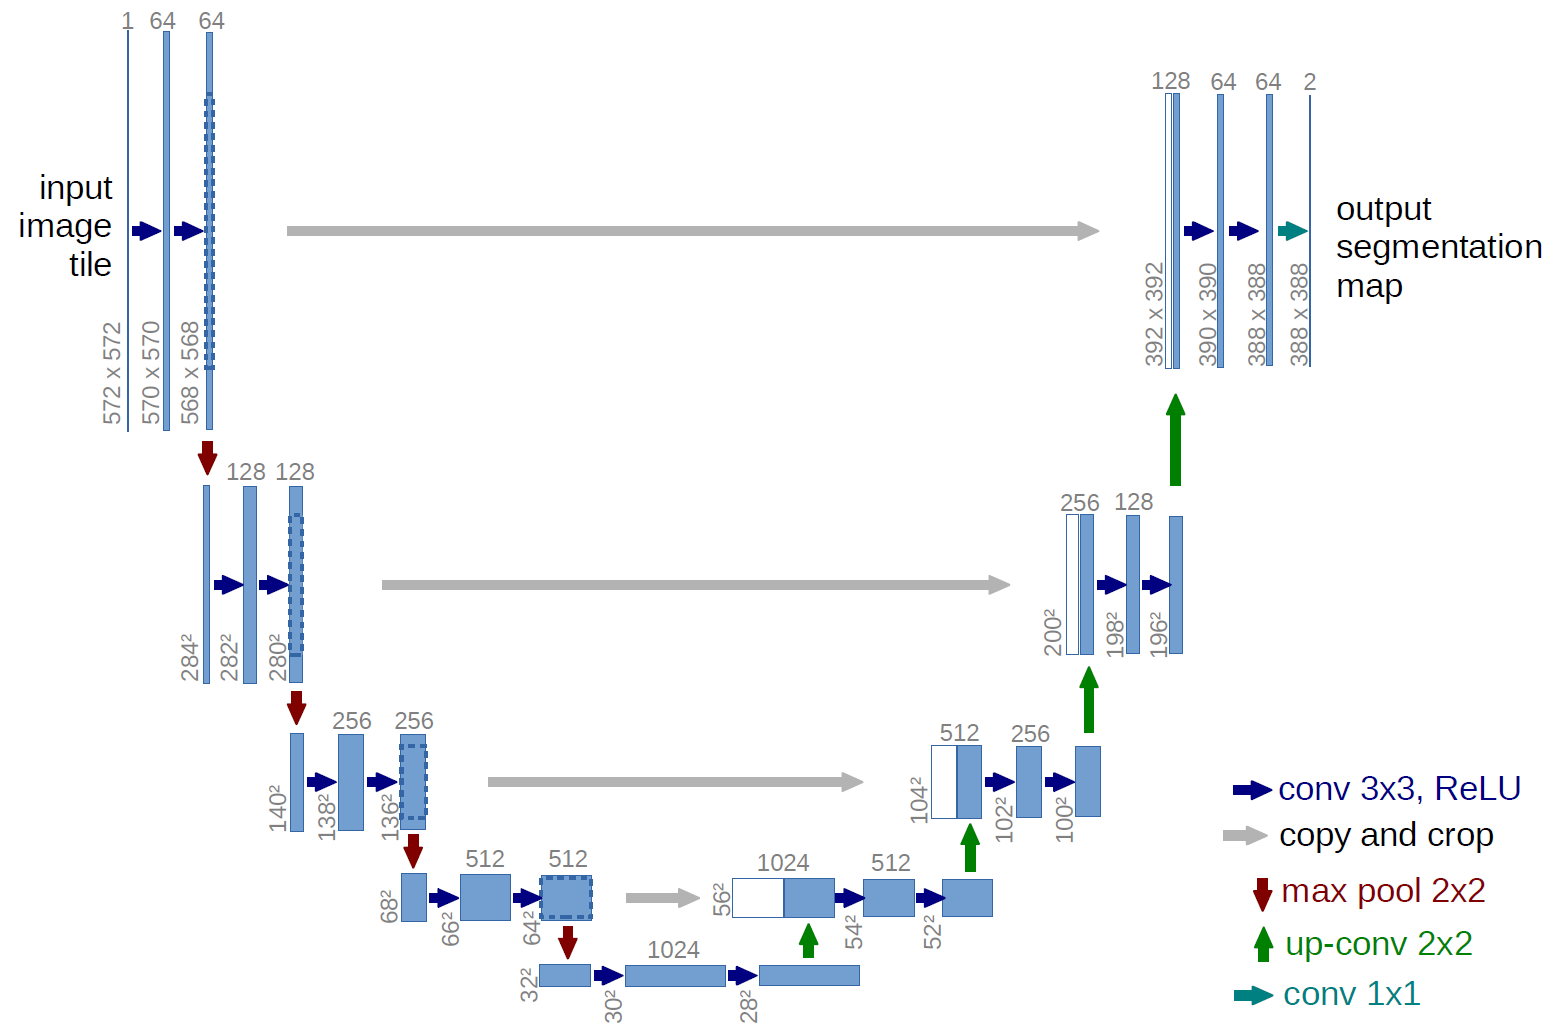
\includegraphics[width=0.8\linewidth]{u-net-architecture.png}
    \caption{U-Net Architecture}
    \label{fig:unet}
\end{figure}
U-net is a convolution neural network developed at the Computer Science Department of the University of Freiburg. It is called U-net, as the network architecture is shaped in a ‘U’. This represents the max-pooling layers and up scaling layers in the network, which represent a contracting and expanding path, respectively. This model makes use of valid convolutions. U-net has shown great performance in image segmentation task, such as vessels in the retina, and liver and tumor in CT scans. High performance in these fields led to the implementation of U-net in HC segmentation. In case of our implementation, the Adam optimizer was used, with a learning rate of 1e - 4 The standard binary cross-entropy loss was chosen for optimization. A second (custom) loss function was experimented with as well, to better represent the loss function used in the COVID-19 segmentation task.
\section{Experiment}
We utilize their pre-divided train, test, and valid set. The U-Net is then trained for 90 epochs and evaluate at the end of each epoch.

The output from the training set and valid set after each epochs are shown in Fig.\ref{fig:train outputs} and Fig.\ref{fig:test outputs}
\begin{figure}[H]
    \centering
    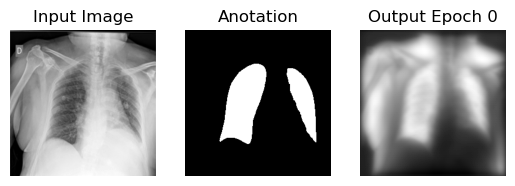
\includegraphics[width=\linewidth]{Unknown-26.png}
    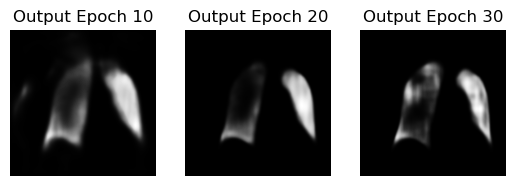
\includegraphics[width=\linewidth]{Unknown-27.png}
    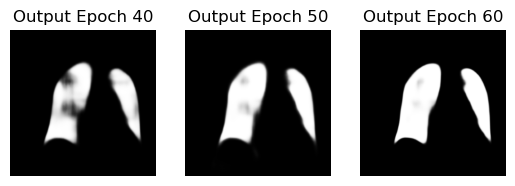
\includegraphics[width=\linewidth]{Unknown-28.png}
    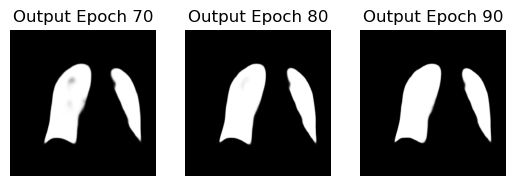
\includegraphics[width=\linewidth]{Unknown-29.png}
    \caption{Train Output in Each Epoch}
    \label{fig:train outputs}
\end{figure}
\begin{figure}[H]
    \centering
    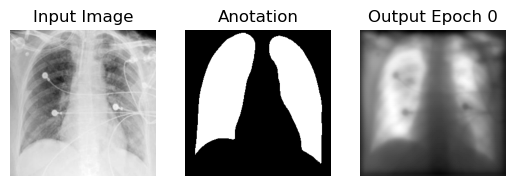
\includegraphics[width=\linewidth]{Unknown-31.png}
    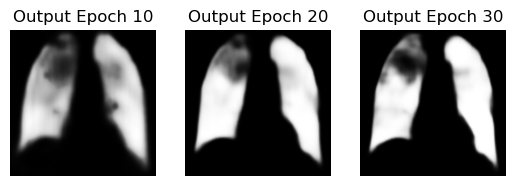
\includegraphics[width=\linewidth]{Unknown-32.png}
    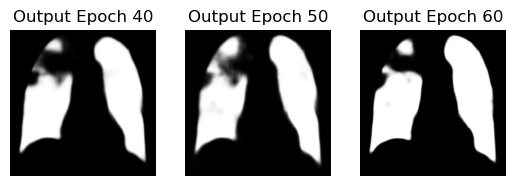
\includegraphics[width=\linewidth]{Unknown-33.png}
    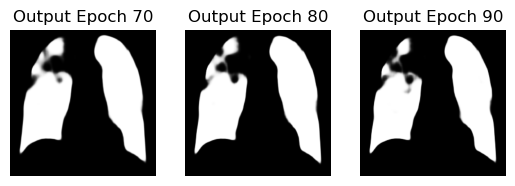
\includegraphics[width=\linewidth]{Unknown-34.png}
    \caption{Test Output in Each Epoch}
    \label{fig:test outputs}
\end{figure}
The train and valid loss progression can be seen in Fig.\ref{fig:loss}
\begin{figure}[H]
    \centering
    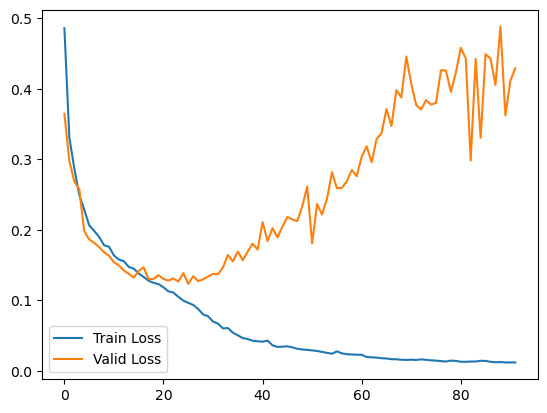
\includegraphics[width=\linewidth]{Unknown-30.png}
    \caption{Training and Validating Loss Progression}
    \label{fig:loss}
\end{figure}

\end{multicols}
\end{document}
